\uuid{qyuH}
\exo7id{5007}
\titre{exo7 5007}
\auteur{quercia}
\organisation{exo7}
\datecreate{2010-03-17}
\isIndication{false}
\isCorrection{true}
\chapitre{Courbes planes}
\sousChapitre{Branches infinies}
\module{Géométrie}
\niveau{L2}
\difficulte{}

\contenu{
\texte{
Déterminer les branches infinies pour les courbes paramétrées suivantes :
}
\begin{enumerate}
    \item \question{$x=4t^5-4t^3+t$,
$y=\dfrac{t}{3t^4+1}$                                 \par


% %-----------------------------------------------------------------------------
% \vtop to 7cm{\mapleplot{%					img1
% x:=4*t^5-4*t^3+t;
% y:=t/(3*t^4+1);
% print(plot([x,y,t=-2..2],-3..3,numpoints=200));}      \par
% \vss}}
\reponse{$$
\centerline{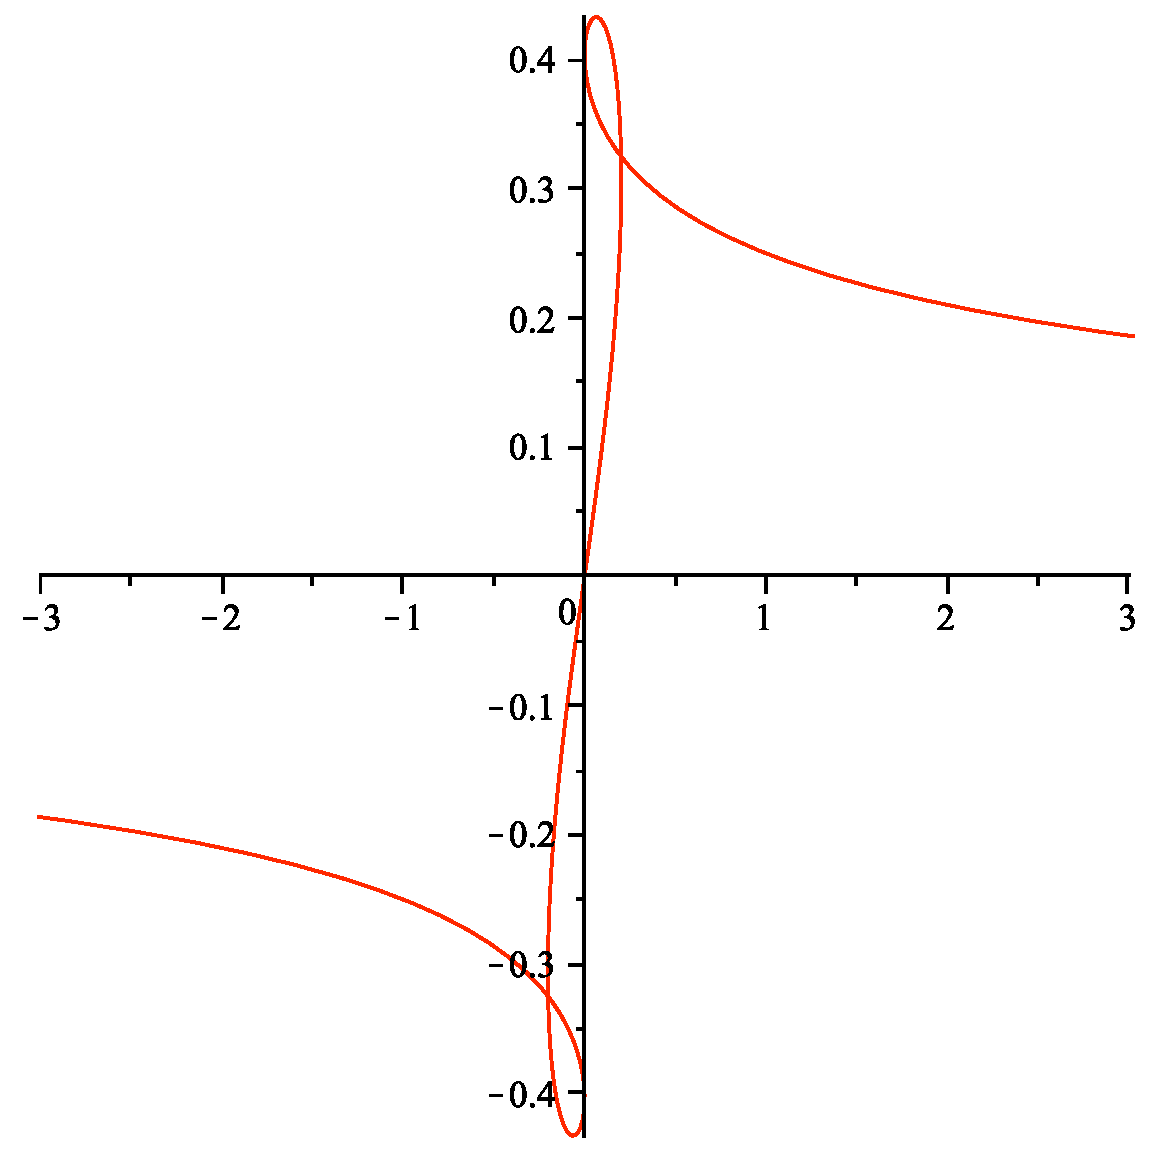
\includegraphics[height=4cm]{../images/pdf/qyuH-1.pdf}}
$$}
    \item \question{$x=2\cos^2t+\ln|\sin t|$,
 $y=\sin 2t$        \par

% %-----------------------------------------------------------------------------
% \vtop to 7cm{\mapleplot{%					img2
% x:=2*cos(t)^2+ln(abs(sin(t)));
% y:=sin(2*t);
% print(plot([x,y,t=0..Pi],-2..2,scaling=constrained));}  \par
                                     
                                     % \vss}}
\reponse{$$
\centerline{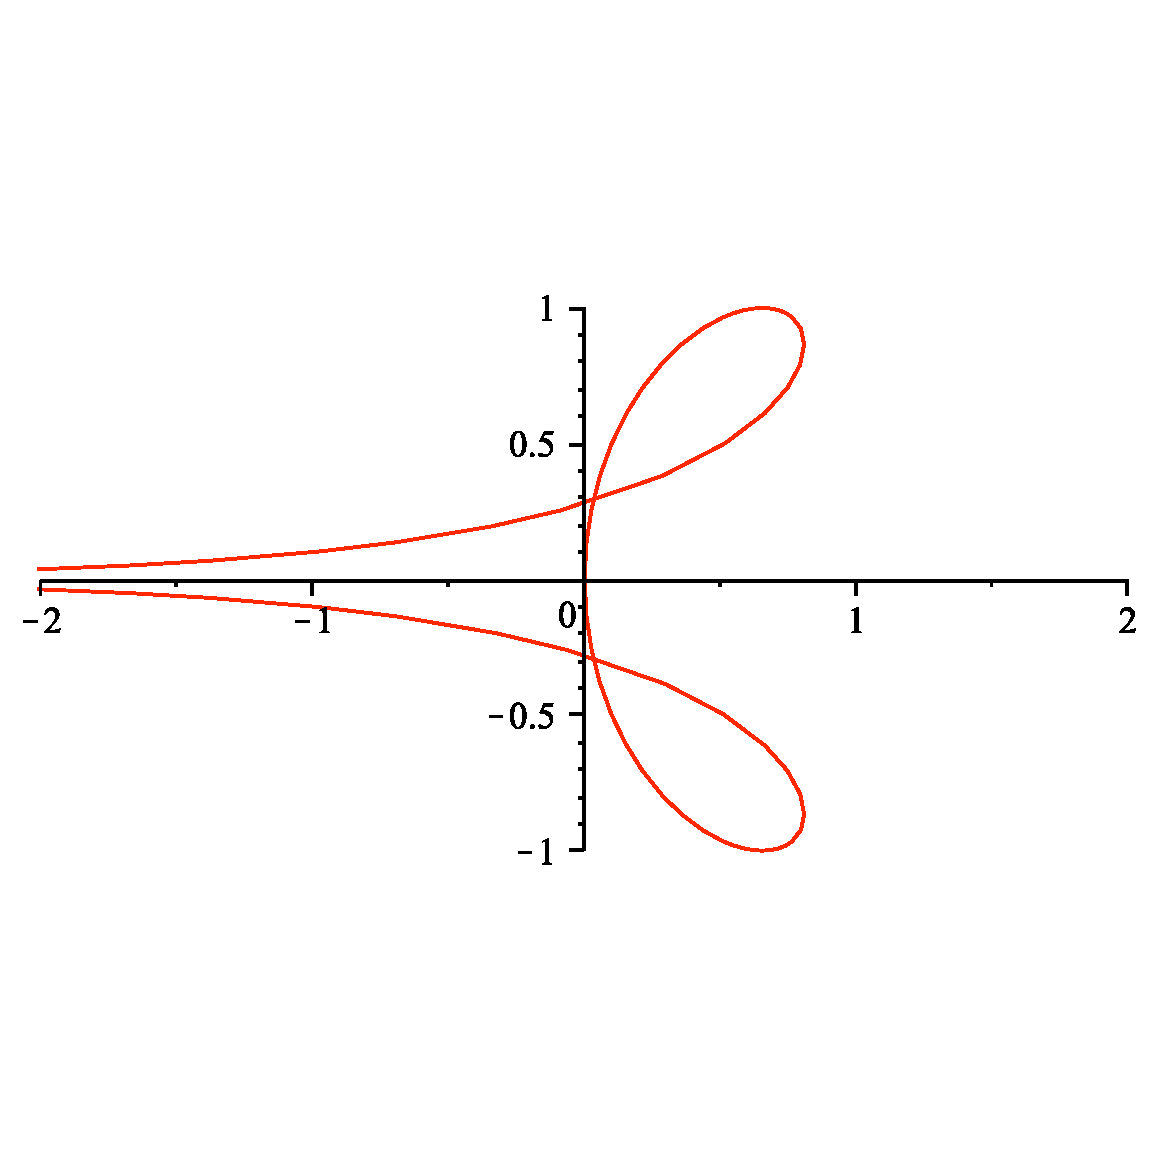
\includegraphics[height=4cm]{../images/pdf/qyuH-2.pdf}}
$$}
    \item \question{$x=\sqrt{\dfrac{t^2-2}{t^4-1}}$,
$y=tx$                                                  \par

% %-----------------------------------------------------------------------------
% \vtop to 7cm{\mapleplot{%					img3
% x:=sqrt((t^2-2)/(t^4-1));
% u:=sqrt((1-2*t^2)/(1-t^4));
% p1:=plot([x,t*x,t=-1..1],-2..3,-2..2):
% p2:=plot([t*u,u,t=0..sqrt(1/2)],-2..3,-2..2):
% p3:=plot([t*u,-u,t=0..sqrt(1/2)],-2..3,-2..2):
% p4:=plot([abs(t),t,t=-2..2],-2..3,-2..2,color=yellow):
% with(plots):
% print(display({p1,p2,p3,p4}));}                         \par
% \vss}}
\reponse{$$
\centerline{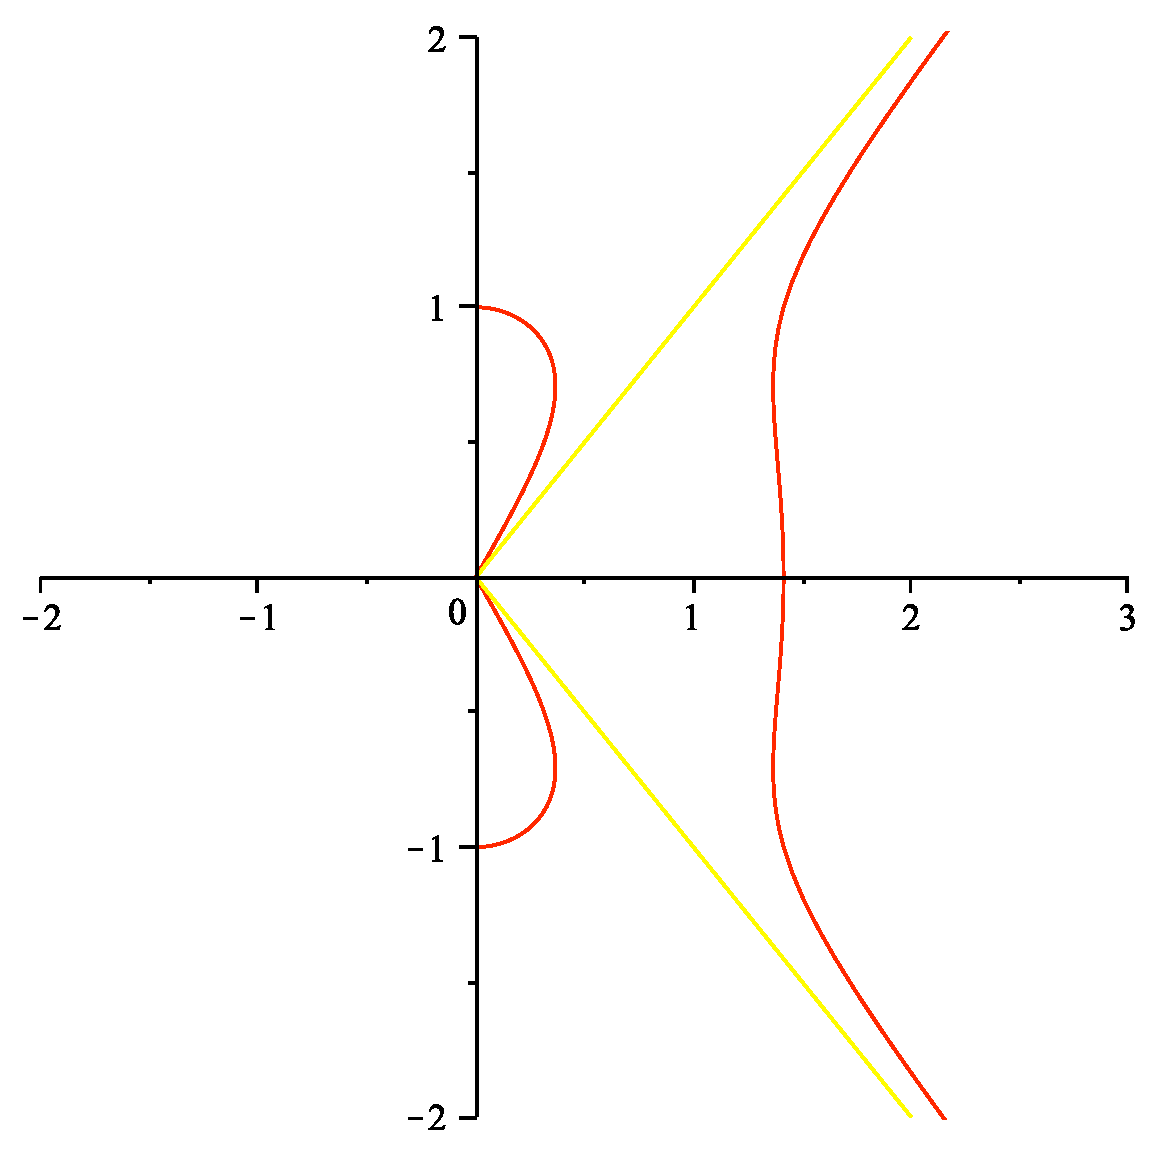
\includegraphics[height=4cm]{../images/pdf/qyuH-3.pdf}}
$$
asymptotes : $y=\pm x$                                  \par
$x-y \sim 1/(4x)  \Rightarrow $ aire infinie                      \par
$y'=0 \Leftrightarrow t=0,(\sqrt6\pm\sqrt2)/2$                     \par}
    \item \question{$x=\dfrac{t^3-t}{2t-1}$,
 $y=tx$                                                   \par

% %-----------------------------------------------------------------------------
% \vtop to 7cm{\mapleplot{%					img4
% x:=(t^3-t)/(2*t-1);
% y:=t*x;
% print(plot([x,y,t=-2..2],-1..1,-1..1));}                 \par
% \vss}}
\reponse{$$
\centerline{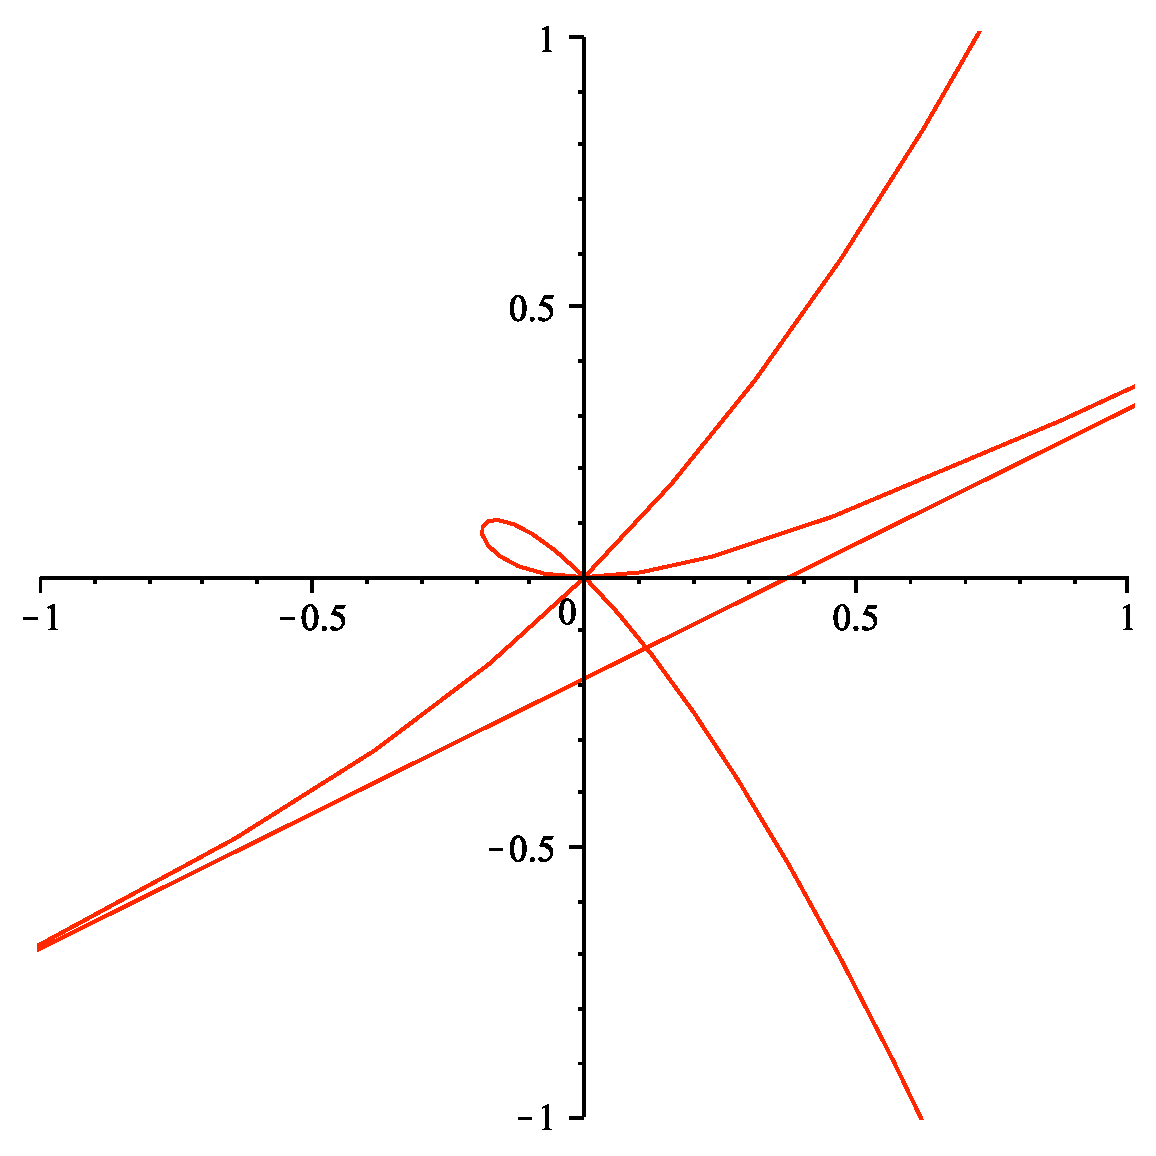
\includegraphics[height=4cm]{../images/pdf/qyuH-4.pdf}}
$$
asymptote : $y=\frac x2 - \frac 3{16}$ (traversée)     \par}
    \item \question{$x=\dfrac1t+\dfrac1{t+1}$, $y=\dfrac1t+\dfrac1{(t+1)^2}$                            \par
% %-----------------------------------------------------------------------------
% \vtop to 7cm{\mapleplot{%					img5
% x:=1/t+1/(t+1);
% y:=1/t+1/(t+1)^2;
% print(plot([x,y,t=-10..10],-4..4,-3..3,numpoints=200));} \par
% \vss}}
\reponse{$$
\centerline{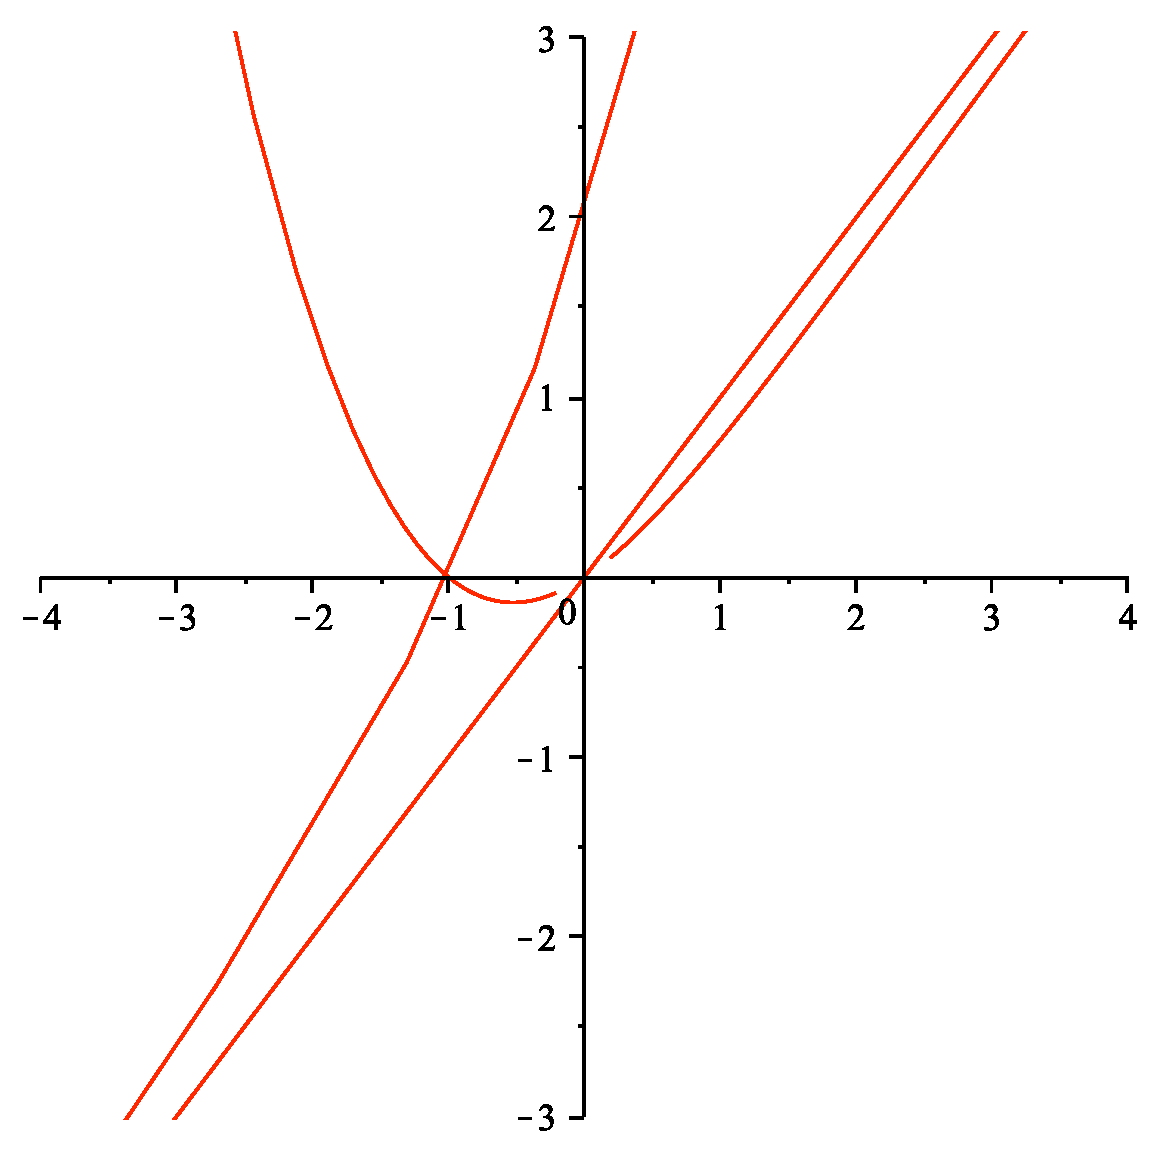
\includegraphics[height=4cm]{../images/pdf/qyuH-5.pdf}}
$$
asymptote : $y=x$                                        \par}
    \item \question{$x=\sin \dfrac t2$,
 $y=\tan t$                                               \par
% %-----------------------------------------------------------------------------
% \vtop to 7cm{\mapleplot{%					img6
% x:=sin(t/2);
% y:=tan(t);
% print(plot([x,y,t=0..4*Pi],-1.5..1.5,-2..2));}           \par
% \vss}\endmulticolonne
% 
% \vfill\eject
% \vphantom{\Gros\bf Branches infinies}\SV\multicolonne 2}
\reponse{$$
\centerline{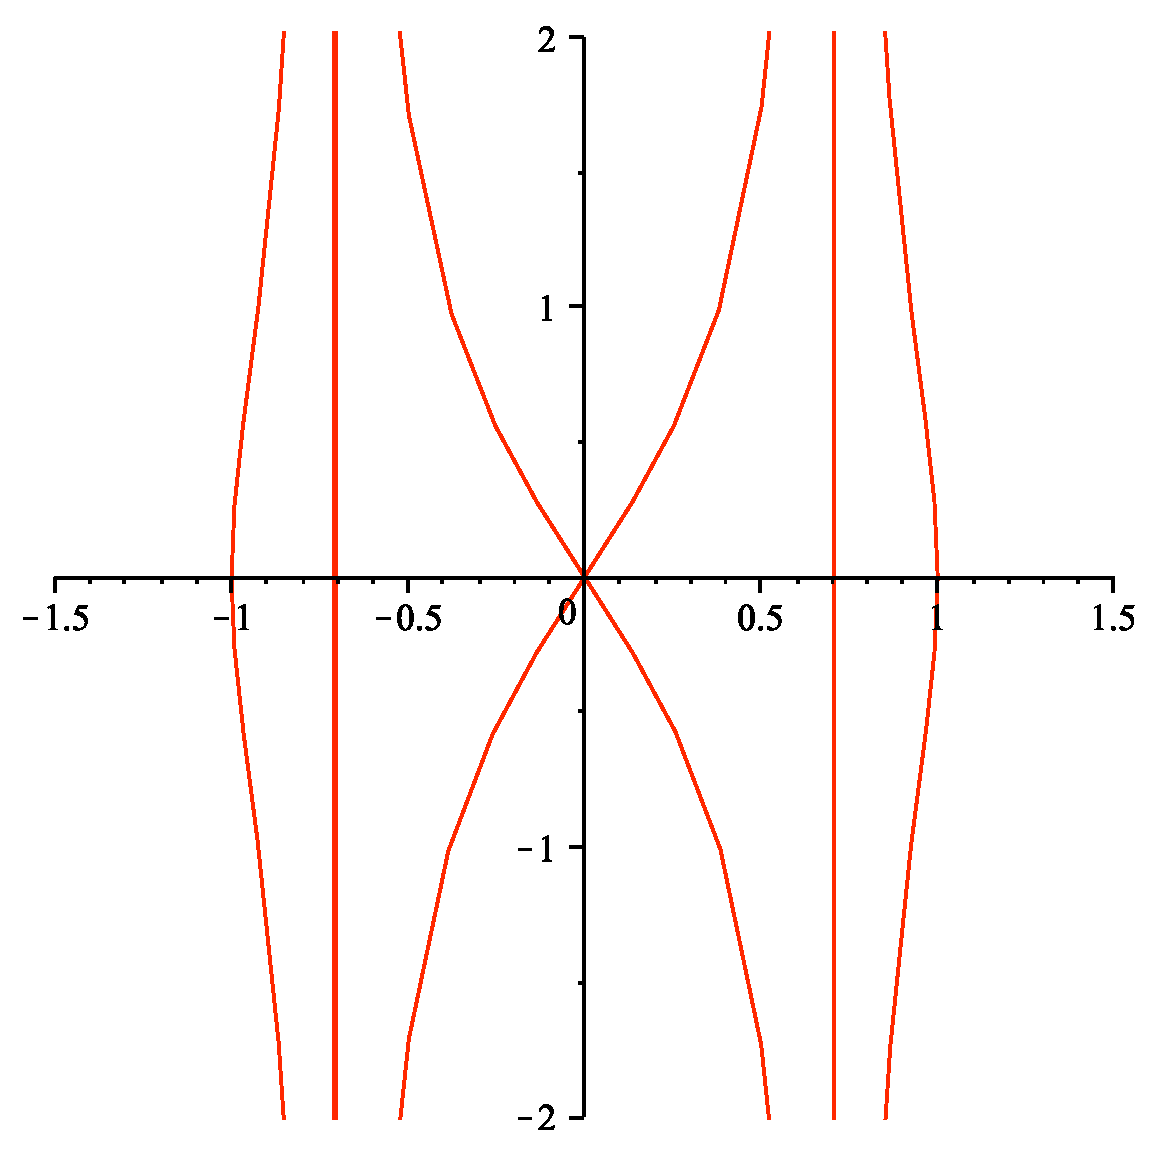
\includegraphics[height=4cm]{../images/pdf/qyuH-6.pdf}}
$$
inflexions : $\tan\frac t2 = 0,\pm3$                    \par}
    \item \question{$x=\dfrac1t+\dfrac1{t+1}$,
 $y=\dfrac1t-\dfrac1{t+1}$                                \par
% %-----------------------------------------------------------------------------
% \vtop to 7cm{\mapleplot{%					img7
% x:=1/t+1/(t+1);
% y:=1/t-1/(t+1);
% print(plot([x,y,t=-5..5],-7..7,-6..4,numpoints=200));}   \par
% \vss}}
\reponse{$$
\centerline{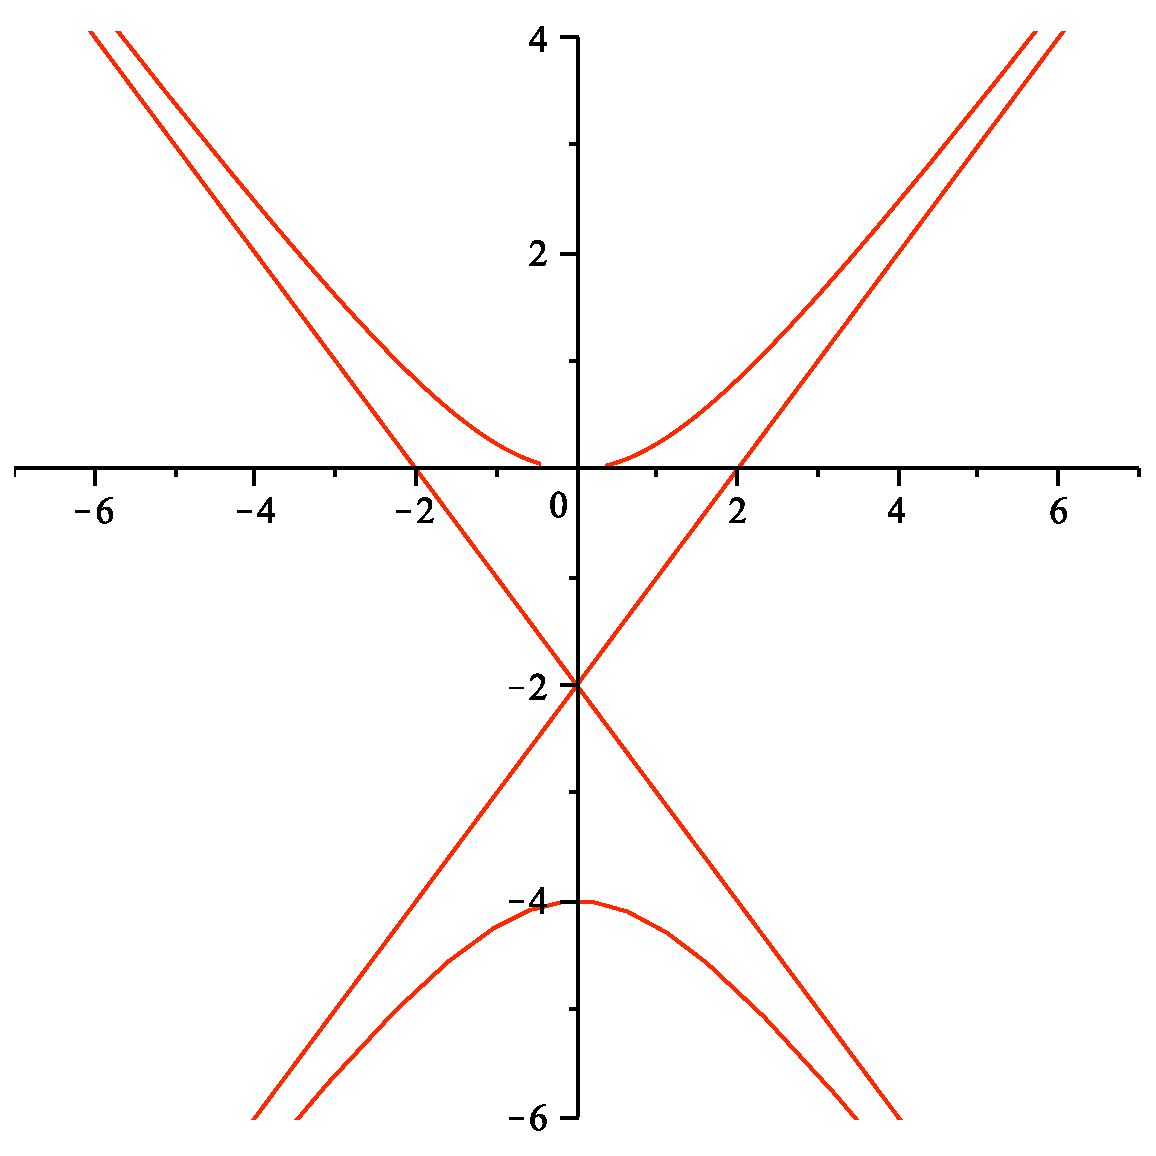
\includegraphics[height=4cm]{../images/pdf/qyuH-7.pdf}}
$$
hyperbole : $(y+2)^2-x^2=4$                              \par}
    \item \question{$x=\dfrac{3t}{1+t^3}$,
 $y=tx$                                                   \par
% %-----------------------------------------------------------------------------
% \vtop to 7cm{\mapleplot{%					img8
% x:=(3*t)/(1+t^3);
% y:=t*x;
% print(plot([x,y,t=-10..10],-4..4,-3..3));}               \par
% \vss}}
\reponse{$$
\centerline{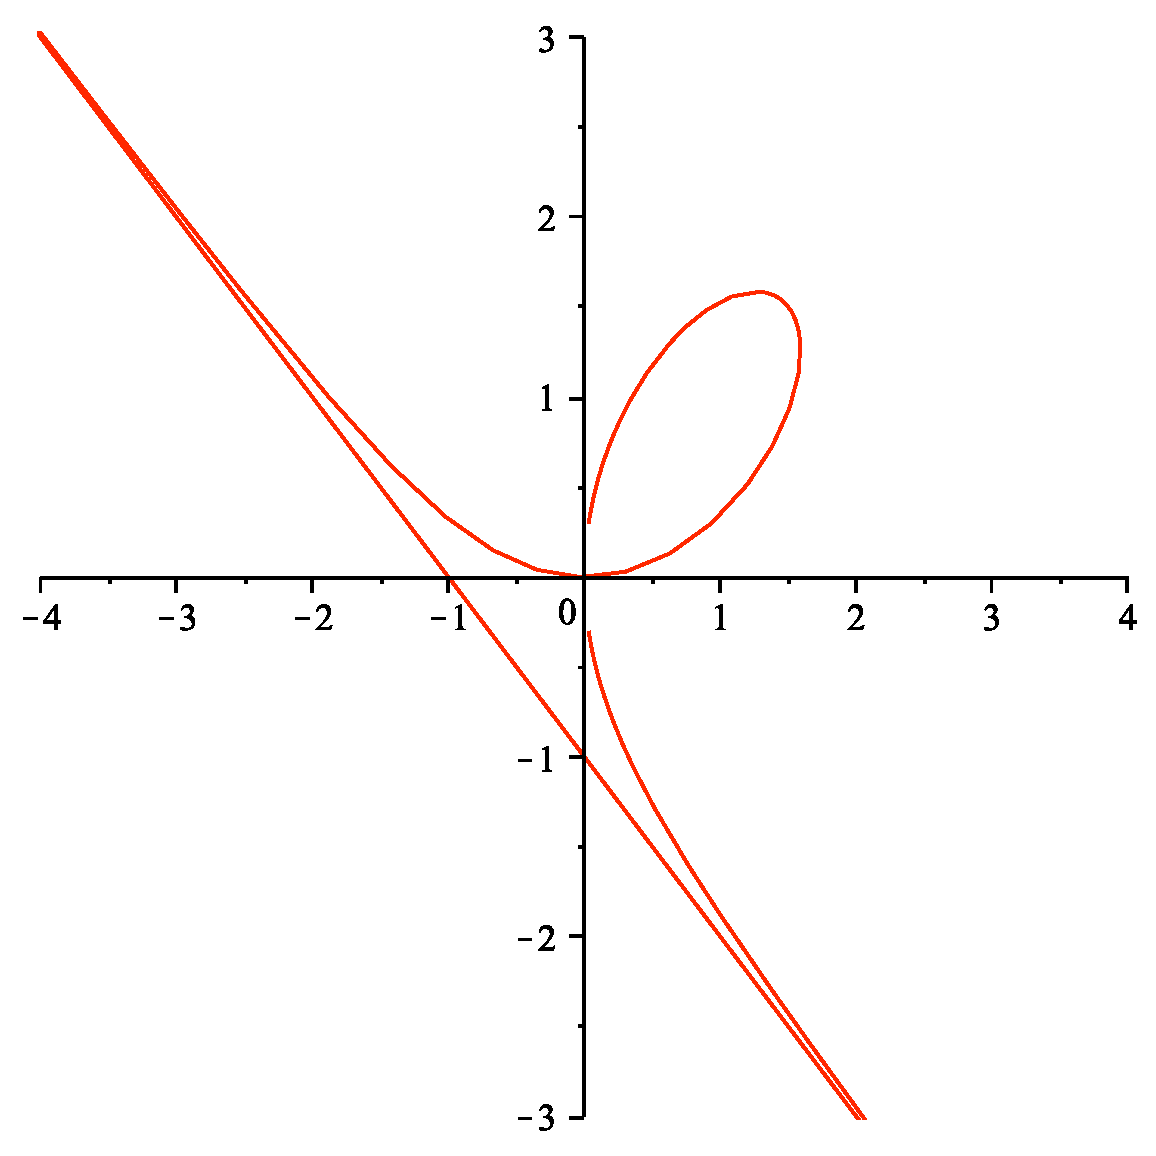
\includegraphics[height=4cm]{../images/pdf/qyuH-8.pdf}}
$$
asymptote : $x+y=-1$                                     \par
équation cartésienne : $x^3+y^3=3xy$                     \par}
    \item \question{$x=\dfrac{te^t}{t+1}$,
 $y=\dfrac{e^t}{t+1}$                                     \par
% %-----------------------------------------------------------------------------
% \vtop to 7cm{\mapleplot{%					img9
% y:=exp(t)/(t+1);
% x:=t*y;
% print(plot([x,y,t=-5..3],-4..4,-3..3));}                 \par
% \vss}}
\reponse{$$
\centerline{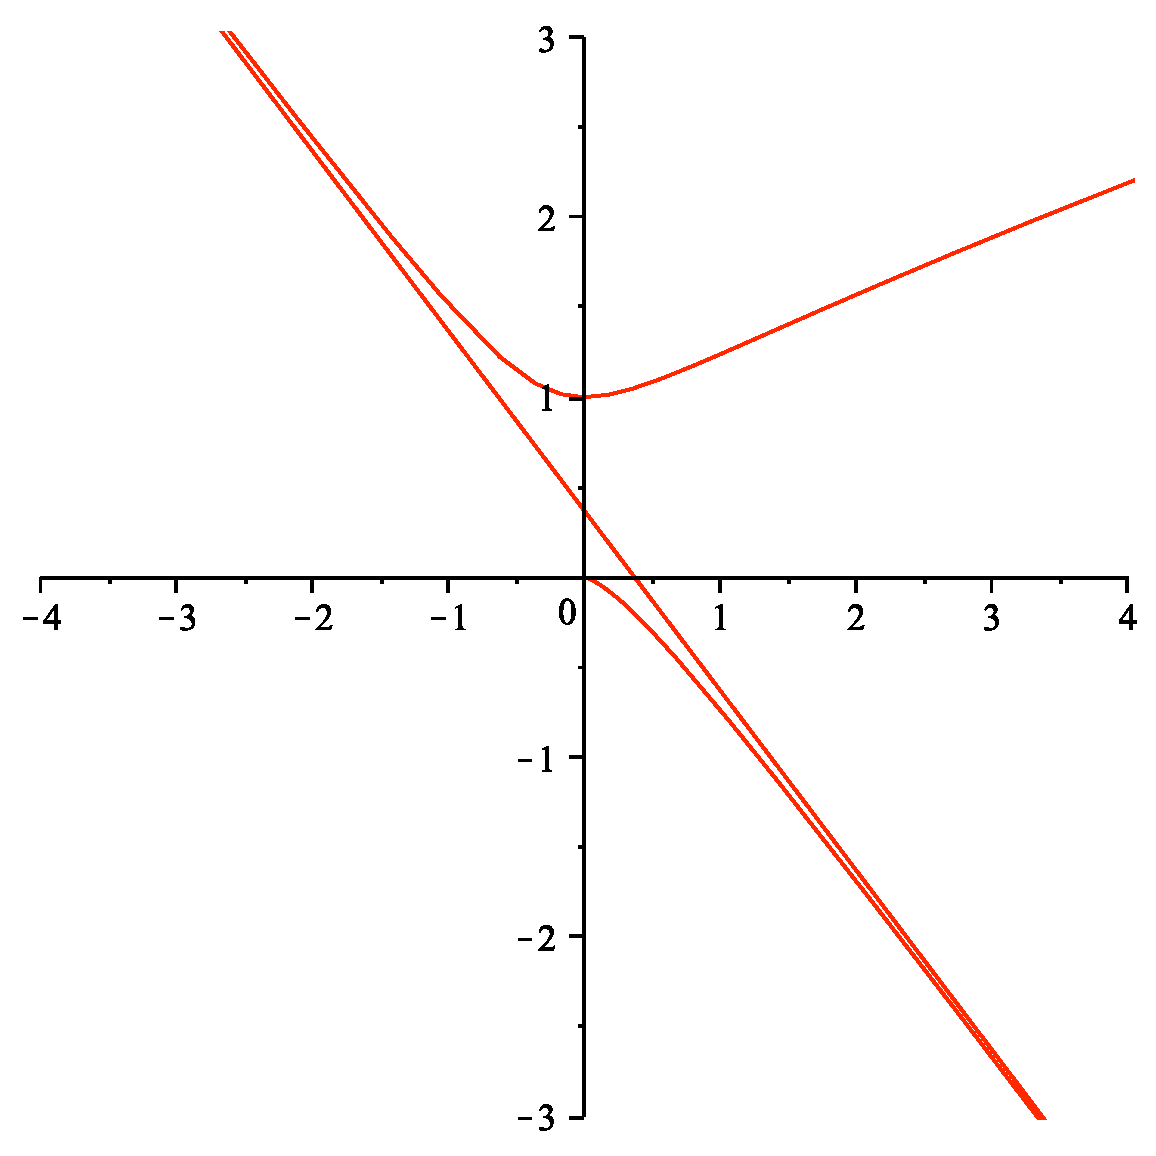
\includegraphics[height=4cm]{../images/pdf/qyuH-9.pdf}}
$$
asymptote : $x+y=e^{-1}$                                 \par
branche parabolique horizontale}
    \item \question{$x=2t^3+3t^2$,
$y=3t^2+6t$                                              \par
% %-----------------------------------------------------------------------------
% \vtop to 7cm{\mapleplot{%					img10
% x:=2*t^3+3*t^2;
% y:=3*t^2+6*t;
% print(plot([x,y,t=-5..5],-50..50,-2..50));}              \par
% \vss}}
\reponse{$$
\centerline{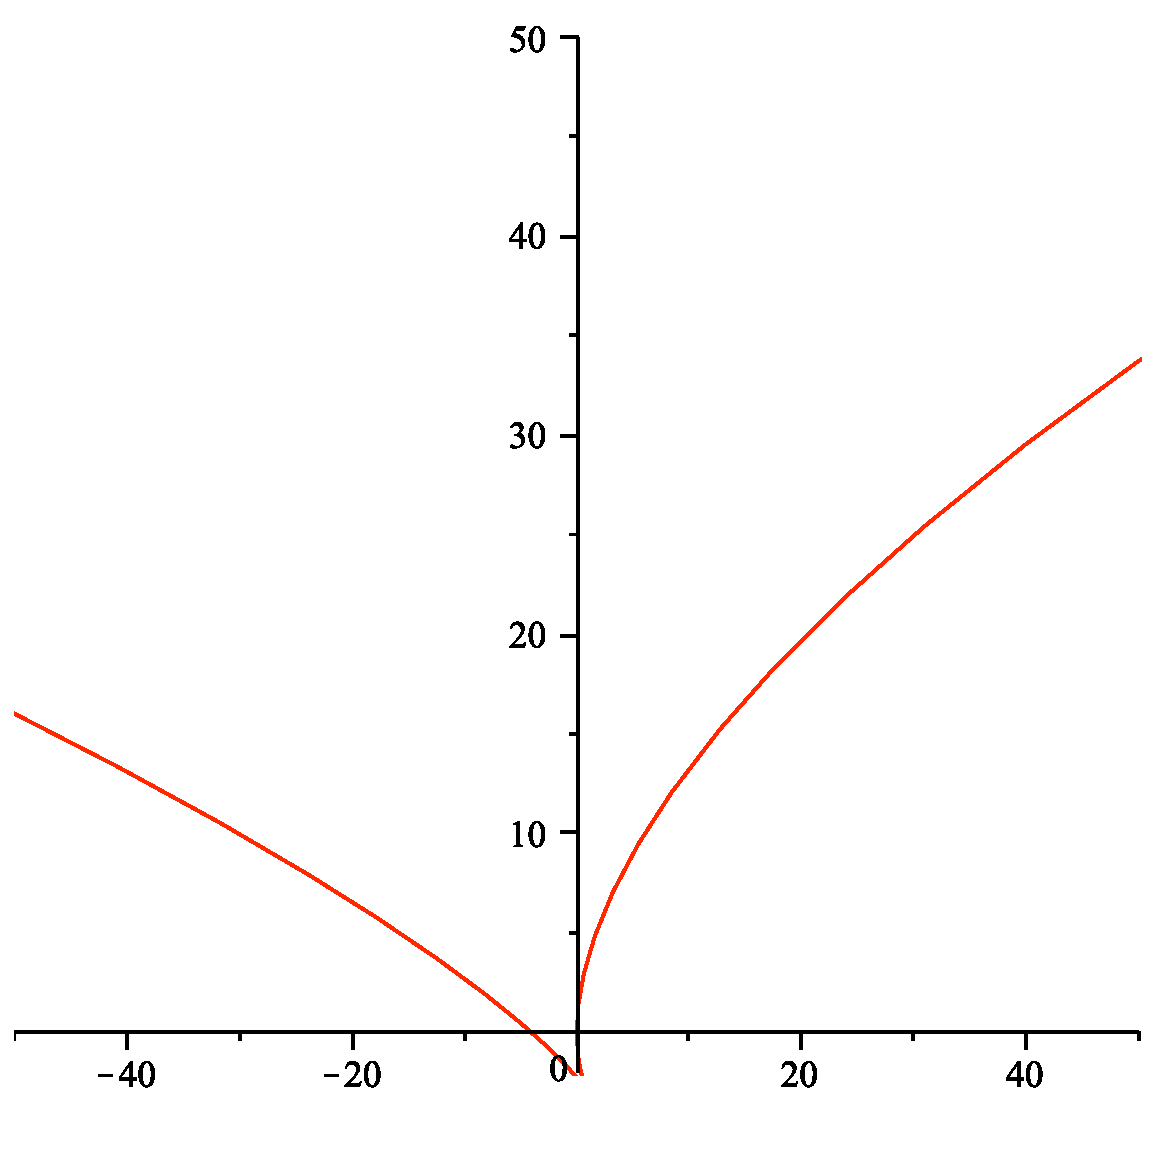
\includegraphics[height=4cm]{../images/pdf/qyuH-10.pdf}}
$$
branche parabolique horizontale                          \par
rebroussement pour $t=1$                                 \par}
    \item \question{$x=t^3-3t$,               
$y=t^3-t^2-t+1$                                          \par
% %-----------------------------------------------------------------------------
% \vtop to 7cm{\mapleplot{%					img11
% x:=t^3-3*t;
% y:=t^3-t^2-t+1;
% print(plot([x,y,t=-3..3],-10..10,-7..7));}               \par
% \vss}}
\reponse{$$
\centerline{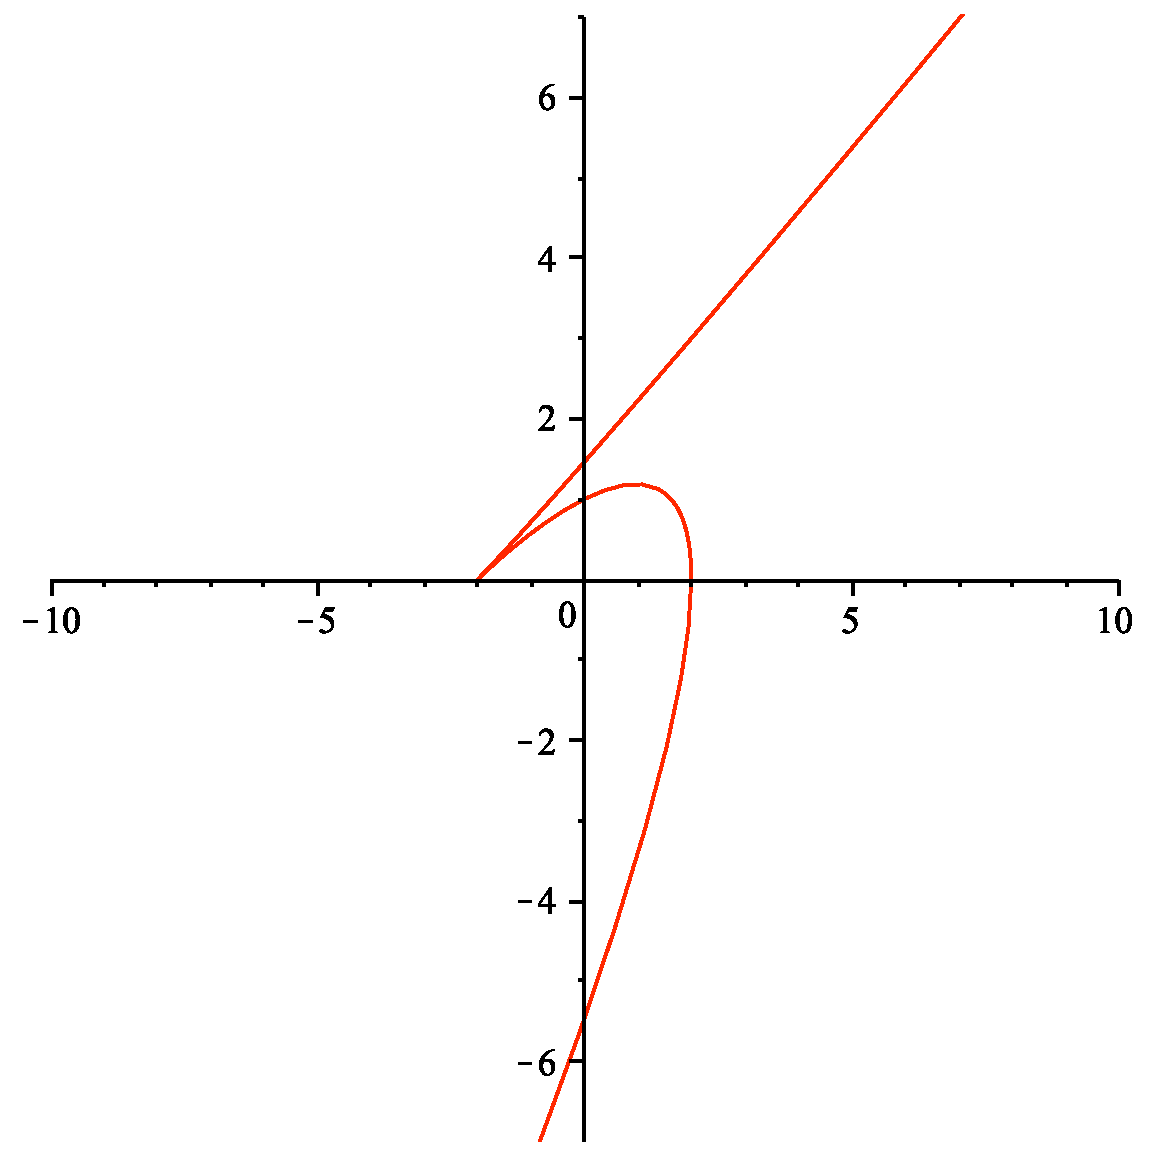
\includegraphics[height=4cm]{../images/pdf/qyuH-11.pdf}}
$$
branche parabolique de coefficient 1                     \par}
    \item \question{$x=\dfrac t{t^2-1}$, 
$y=\dfrac{t^2}{t-1}$                                     \par
% %-----------------------------------------------------------------------------
% \vtop to 7cm{\mapleplot{%					img12
% x:=t/(t^2-1);
% y:=t^2/(t-1);
% print(plot([x,y,t=-5..5],-4..4,-3..5));}                 \par
% \vss}}
\reponse{$$
\centerline{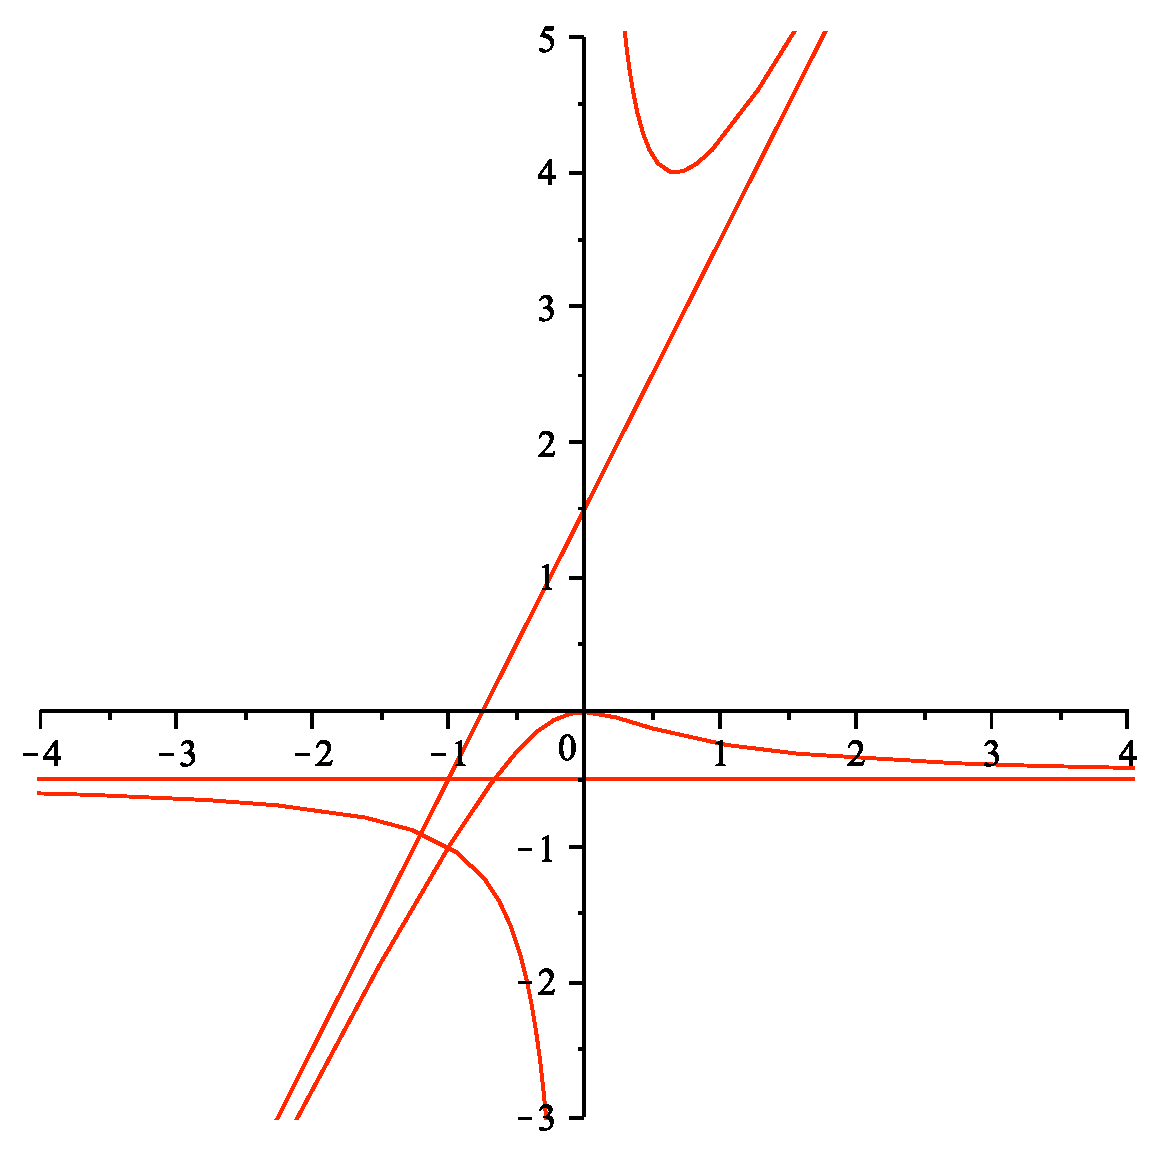
\includegraphics[height=4cm]{../images/pdf/qyuH-12.pdf}}
$$
 asymptote : $y=2x+\frac 32$                              \par
 point double : $t^2+t=1$, $x=y=-1$
 les tangentes sont orthogonales}
\end{enumerate}
}
